%%%%%%%%%%%%%%%%%%%%%%%%%%%%%%%%%%%%%%%%%%%%%%%%%%%%%%%%%%%%%%%%%%%%%%%%%%%

\documentclass{standalone}

\usepackage{amsmath}
\usepackage{mathptmx}
\usepackage{pgfplots}
\usetikzlibrary{external}
\tikzexternalize{inverses}
\pgfplotsset{compat=1.15}

%% IEEE uses Times Roman font, so we'll default to Times.
%% These three commands make up the entire times.sty package.
\renewcommand{\rmdefault}{ptm}
\renewcommand{\ttdefault}{pcr}
\normalfont\selectfont

\newcommand{\comma}{,\,}
\newcommand{\tuple}[2]{\left({#1}\comma {#2}\right)}

\begin{document}

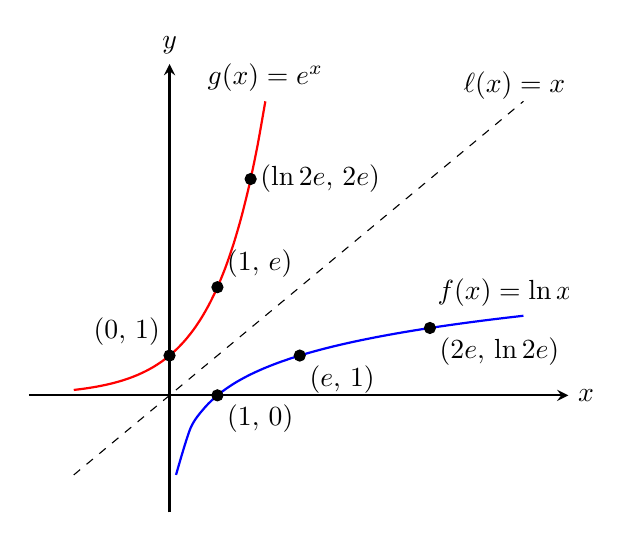
\begin{tikzpicture}
\tikzset{%%
  every mark/.append style={scale=1.0},%%
  scale=1.0%%
}
\pgfplotsset{%%
  every axis/.append style={font=\normalsize}%%
}
%%
\begin{axis}[%%
  axis line style=thick,%%
  axis lines=center,%%
  dotStyle/.style={only marks,mark size=2,black,mark color=black,mark=*},%%
  enlargelimits=true,%%
  plotStyle/.style={%%
    mark=none,%%
    smooth,%%
    thick%%
  },%%
  ticks=none,%%
  %% x axis
  xlabel={\normalsize $x$},%%
  xlabel style=right,%%
  %% y axis
  ylabel={\normalsize $y$},%%
  ylabel style=above%%
]
%%
%%
%% The natural logarithmic function.
\addplot+ [plotStyle,domain=0.135335283236613:7.38905609893065,blue]
{ln(x)};
%% Label the above functions.
\node[above] at (axis cs:7,2) {$f(x) = \ln x$};
%% Add some points on the graph of the logarithmic function.
\addplot[dotStyle] coordinates {
  (1,0)
  (2.71828182845905,1)
  (5.43656365691809,1.69314718055995)
};
%% Label the above points.
\node[below right] at (axis cs:1,0) {$\tuple{1}{0}$};
\node[below right] at (axis cs:2.71828182845905,1) {$\tuple{e}{1}$};
\node[below right] at (axis cs:5.43656365691809,1.69314718055995) {$\tuple{2e}{\ln 2e}$};
%%
%%
%% The exponential function.
\addplot+ [plotStyle,domain=-2:2,red]
{exp(x)};
%% Label the above functions.
\node[above] at (axis cs:2,7.38905609893065) {$g(x) = e^x$};
%% Add some points on the graph of the exponential function.
\addplot[dotStyle] coordinates {
  (0,1)
  (1,2.71828182845905)
  (1.69314718055995,5.43656365691809)
};
%% Label the above points.
\node[above left] at (axis cs:0,1) {$\tuple{0}{1}$};
\node[above right] at (axis cs:1,2.71828182845905) {$\tuple{1}{e}$};
\node[right] at (axis cs:1.69314718055995,5.43656365691809) {$\tuple{\ln 2e}{2e}$};
%%
%%
%% The linear functinon f(x) = x.
\addplot+ [plotStyle,domain=-2:7.38905609893065,black,dashed,thin]
{x};
%% Label the above functions.
\node[above] at (axis cs:7.2,7.2) {$\ell(x) = x$};
\end{axis}
\end{tikzpicture}

\end{document}
